\documentclass{article}

\usepackage{fullpage}
\usepackage{color}
\usepackage{amsmath}
\usepackage{url}
\usepackage{verbatim}
\usepackage{graphicx}
\usepackage{parskip}
\usepackage{amssymb}
\usepackage{nicefrac}
\usepackage{listings} % For displaying code
\usepackage{algorithm2e} % pseudo-code

% Answers
\def\ans#1{\par\gre{Answer: #1}}

% Colors
\definecolor{blu}{rgb}{0,0,1}
\def\blu#1{{\color{blu}#1}}
\definecolor{gre}{rgb}{0,.5,0}
\def\gre#1{{\color{gre}#1}}
\definecolor{red}{rgb}{1,0,0}
\def\red#1{{\color{red}#1}}
\def\norm#1{\|#1\|}

% Math
\def\R{\mathbb{R}}
\def\argmax{\mathop{\rm arg\,max}}
\def\argmin{\mathop{\rm arg\,min}}
\newcommand{\mat}[1]{\begin{bmatrix}#1\end{bmatrix}}
\newcommand{\alignStar}[1]{\begin{align*}#1\end{align*}}
\def\cond{\; | \;} 

% LaTeX
\newcommand{\fig}[2]{\includegraphics[width=#1\textwidth]{a2f/#2}}
\newcommand{\centerfig}[2]{\begin{center}\includegraphics[width=#1\textwidth]{a2f/#2}\end{center}}
\def\items#1{\begin{itemize}#1\end{itemize}}
\def\enum#1{\begin{enumerate}#1\end{enumerate}}
\newcommand{\matCode}[1]{\lstinputlisting[language=Matlab]{a2f/#1.m}}


\begin{document}

\title{CPSC 340 Assignment 2 (due Friday September 27 at 11:55pm)}
\author{}
\date{}
\maketitle
\vspace{-4em}

The assignment instructions are the same as Assignment 1, except you have the option to work in a group of 2. If you work in a group, please only hand in \emph{one} assignment. It is recommended that you work in groups as the assignment is quite long, but please only submit one assignment for the group and make sure that everyone's name/ID is on the front page.



\section{Training and Testing}

\subsection{Traning Error}

Running \texttt{example\_train.jl} fits decision trees of different depths using two different implementations:
the ``decisionStump'' function from Assignment 1, and using a variant using a more sophisticated splitting criterion called the information gain. \blu{Describe what you observe. Can you explain the results?}
\ans{The result shows the accuracy based decision tree have an lower bound on the training error of 0.11, but the information gain based decision tree can successfully classify all the sample in the training set (training error = 0).\\
However, if the depth of the tree is shallow (depth <= 4 here), the training error of the information gain based tree have a higher training error.}



\subsection{Training and Testing Error Curves}

Notice that the \emph{citiesSmall.mat} file also contains test data, ``Xtest" and ``ytest". 
Running \emph{example\_trainTest} trains a depth-2 decision tree and evaluates its performance on the test data. %\footnote{The code uses the "information gain" splitting criterion; see the Decision Trees bonus slides for more information.} 
With a depth-2 decision tree, the training and test error are fairly close, so the model hasn't overfit much.


\blu{Make a plot that contains the training error and testing error as you vary the depth from 1 through 15. How do each of these errors change with the decision tree depth?}
\ans{\\
\includegraphics[width = 10cm]{Q1TrainVSTest2.png}\\
As the depth of the tree increased, the Test Erot decreased first, and reached minimum at depth 8. The training error keeps decreasing after that but the test error increased a bit and settled at 0.095 }

Note: use the provided infogain-based decision tree code from the previous subsection.



\subsection{Validation Set}

Suppose we're in the typical case where we don't have the labels for the test data. In this case, we might instead use a \emph{validation} set. Split the training set into two equal-sized parts: use the first $n/2$ examples as a training set and the second $n/2$ examples as a validation set (we're assuming that the examples are already in a random order). \blu{What depth of decision tree would we pick if we minimized the validation set error? Does the answer change if you switch the training and validation set? How could we use more of our data to  estimate the depth more reliably?}
\ans{\\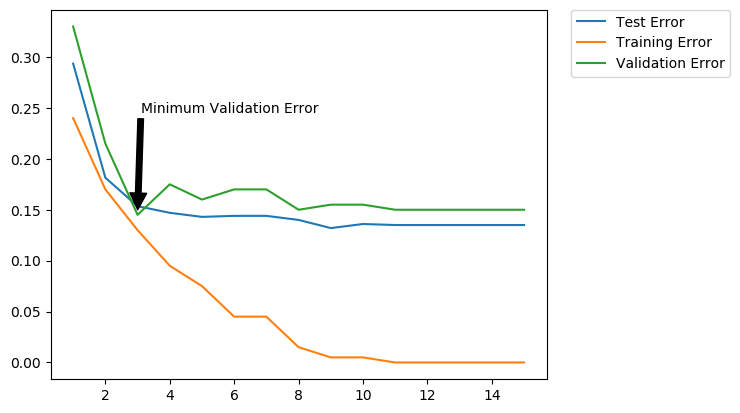
\includegraphics[width = 10cm]{Q1WithValidationError.png}\\
The depth of decision tree is 3.\\
If we swap the training set and validation set:\\
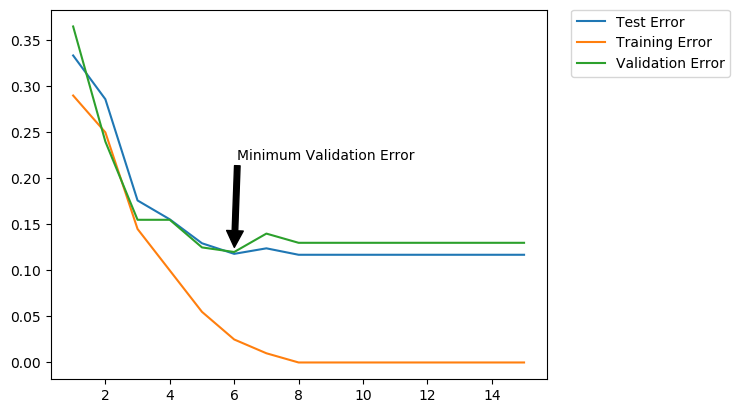
\includegraphics[width = 10cm]{Q1WithValidationErrorReversed.png}
\\The we would pick the depth as 6. The way to use the data is to use k-flod method to test on different validation sets.}
\\Note: use the provided infogain-based decision tree code from the previous subsection.



\section{Naive Bayes}

In this section we'll implement naive Bayes, a very fast classification method that is often surprisingly accurate for text data with simple representations like bag of words.


\subsection{Naive Bayes by Hand}

Consider the dataset below, which has $10$ training examples and $3$ features:
\[
X = \begin{bmatrix}0 & 0 & 1\\0 & 1 & 1\\ 0 & 1 & 1\\ 1 & 1 & 0\\0 & 1 & 0\\0 & 1 & 1\\1 & 0 & 0\\1 & 1 & 0\\1 & 0 & 1\\1 & 0 & 0\\\end{bmatrix}, \quad y = \begin{bmatrix}\text{spam}\\\text{spam}\\\text{spam}\\\text{spam}\\\text{spam}\\\text{spam}\\\text{not spam}\\\text{not spam}\\\text{not spam}\\\text{not spam}\end{bmatrix}.
\]
The feature in the first column is $<$your name$>$ (whether the e-mail contained your name), in the second column is ``pharmaceutical'' (whether the e-mail contained this word), and the third column is ``PayPal'' (whether the e-mail contained this word).
Suppose you believe that a naive Bayes model would be appropriate for this dataset, and you want to classify the following test example:
\[
\hat{x} = \begin{bmatrix}1 & 1 & 0\end{bmatrix}.
\]

\subsubsection{Prior probabilities}

\blu{Compute the estimates of the class prior probabilities} (you don't need to show any work):
\items{
\item$ p(\text{spam})$ \ans {0.6}.
\item $p(\text{not spam})$ \ans{0.4}.
}

\subsubsection{Conditional probabilities}

\blu{Compute the estimates of the 6 conditional probabilities required by naive Bayes for this example}  (you don't need to show any work):
\items{
\item $p(\text{$<$your name$>$} = 1  \cond \text{spam})$. \ans{1/6}
\item $p(\text{pharmaceutical} = 1 \cond \text{spam})$. \ans{5/6}
\item $p(\text{PayPal} = 0  \cond \text{spam})$. \ans{4/6 = 2/3}
\item $p(\text{$<$your name$>$} = 1  \cond \text{not spam})$. \ans{1}
\item $p(\text{pharmaceutical} = 1  \cond \text{not spam})$. \ans{1/4}
\item $p(\text{PayPal} = 0  \cond \text{not spam})$. \ans{1/4}
}

\subsubsection{Prediction}


\blu{Under the naive Bayes model and your estimates of the above probabilities, what is the most likely label for the test example? (Show your work.)}
\ans{\begin{align*} 
    &P(\text{spam} \cond \text{$<$your name$>$} = 1 \& \text{pharmaceutical} = 1 \& \text{PayPal} = 0 ) 
    \\ \approx & \frac{p(\text{$<$your name$>$} = 1  \cond \text{spam}) \times p(\text{pharmaceutical} = 1 \cond \text{spam}) \times p(\text{PayPal} = 0  \cond \text{spam}) \times P(\text{spam})}{C}
    \\ = & \frac{0.6*1/6*5/6*2/3}{C} \\
    =& \frac{1/18}{C}
\end{align*}\\
\begin{align*} 
    &P(\text{not spam} \cond \text{$<$your name$>$} = 1 \& \text{pharmaceutical} = 1 \& \text{PayPal} = 0 ) 
    \\ \approx & \frac{p(\text{$<$your name$>$} = 1  \cond \text{not spam}) \times p(\text{pharmaceutical} = 1 \cond \text{not spam}) \times p(\text{PayPal} = 0  \cond \text{not spam}) \times P(\text{not spam})}{C}
    \\ = & \frac{0.4*1*1/4*1/4}{C} \\
    =& \frac{1/40}{C}
\end{align*}
\\
$ \frac{ P(\text{spam} \cond \text{$<$your name$>$} = 1 \& \text{pharmaceutical} = 1 \& \text{PayPal} = 0 )}{P(\text{not spam} \cond \text{$<$your name$>$} = 1 \& \text{pharmaceutical} = 1 \& \text{PayPal} = 0 )} = \frac{20}{9} > 1$
\\Therefore, the email is more likely to be a spam.}

\subsection{Bag of Words}

If you run the script \emph{example\_bagOfWods.jl}, it will load the following dataset:
\enum{
\item $X$: A sparse binary matrix. Each row corresponds to a newsgroup post, and each column corresponds to whether a particular word was used in the post. A value of $1$ means that the word occured in the post.
\item $wordlist$: The set of words that correspond to each column.
\item $y$: A vector with values $1$ through $4$, with the value corresponding to the newsgroup that the post came from.
\item $groupnames$: The names of the four newsgroups.
\item $Xvalid$ and $yvalid$: the word lists and newsgroup labels for additional newsgroup posts.
}
\blu{Answer the following}:
\enum{
\item Which word is present in the newsgroup post if there is a $1$ in column 30 of X? \ans{format}
\item Which words are present in training example 200? \ans{food, world}
\item Which newsgroup name does training example 200 come from? \ans{talk.*}
}

\subsection{Naive Bayes Implementation}

If you run the function \emph{example\_decisionTree\_newsgroups.jl} it will load the newsgroups dataset and report the test error for decision trees of different sizes (it may take a while for the deeper trees, as this is a sub-optimal implementation). On other other hand, if you run the function \emph{example\_naiveBayes.jl} it will fit the basic naive Bayes model and report the test error.

While the \emph{predict} function of the naive Bayes classifier is already implemented, the calculation of the variable $p\_xy$ is incorrect (right now, it just sets all values to $1/2$). \blu{Modify this function so that \emph{p\_xy} correctly computes the conditional probabilities of these values based on the frequencies in the data set. Hand in your code and report the test error that you obtain.}
\ans{\\ 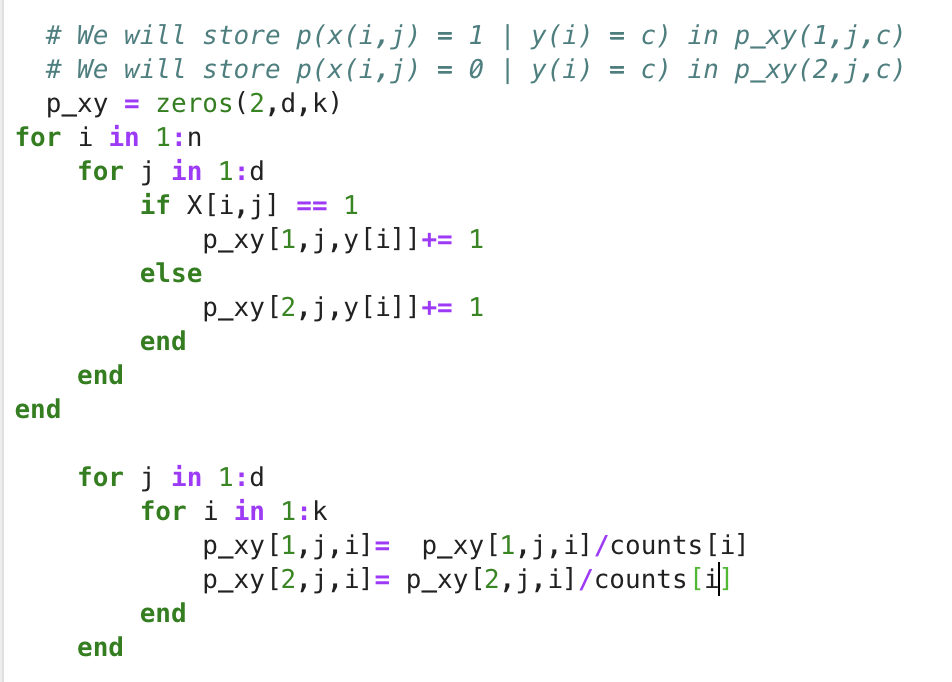
\includegraphics[width = 10cm]{Q2Code2.png}
\\
And the test error is 0.188}

\subsection{Runtime of Naive Bayes for Discrete Data}

Assume you have the following setup:
\items{
\item The training set has $n$ objects each with $d$ features.
\item The test set has $t$ objects with $d$ features.
\item Each feature can have up to $c$ discrete values (you can assume $c \leq n$).
\item There are $k$ class labels (you can assume $k \leq n$)
}
You can implement the training phase of a naive Bayes classifier in this setup in $O(nd)$, since you only need to do a constant amount of work for each $X[i,j]$ value. (You do not have to actually implement it in this way for the previous question, but you should think about how this could be done). \blu{What is the cost of classifying $t$ test examples with the model?}
\ans{
    For ecah test sample, we need to calculate the factor of each y. To do that we need to multiply the probability of all the features in that sample, which is total of d features. That is we need O(kd) for one sample. Therefore, the total cost will be O(kdt).
}



\section{K-Nearest Neighbours}


In \emph{citiesSmall} dataset, nearby points tend to receive the same class label because they are part of the same state. This indicates that a $k-$nearest neighbours classifier might be a better choice than a decision tree (while naive Bayes would probably work poorly on this dataset). The file \emph{knn.jl} has implemented the training function for a $k-$nearest neighbour classifier (which is to just memorize the data) but the predict function always just predicts 1.


\subsection{KNN Prediction}

Fill in the \emph{predict} function in \emph{knn.jl} so that the model file implements the k-nearest neighbour prediction rule. You should use Euclidean distance. 

Hint: although it is not necessary, you may find it useful to pre-compute all the distances (using the \emph{distancesSquared} function in \emph{misc.jl}) and to use the \emph{sortperm} command.
\blu{
\enum{
\item Hand in the predict function. \ans{\\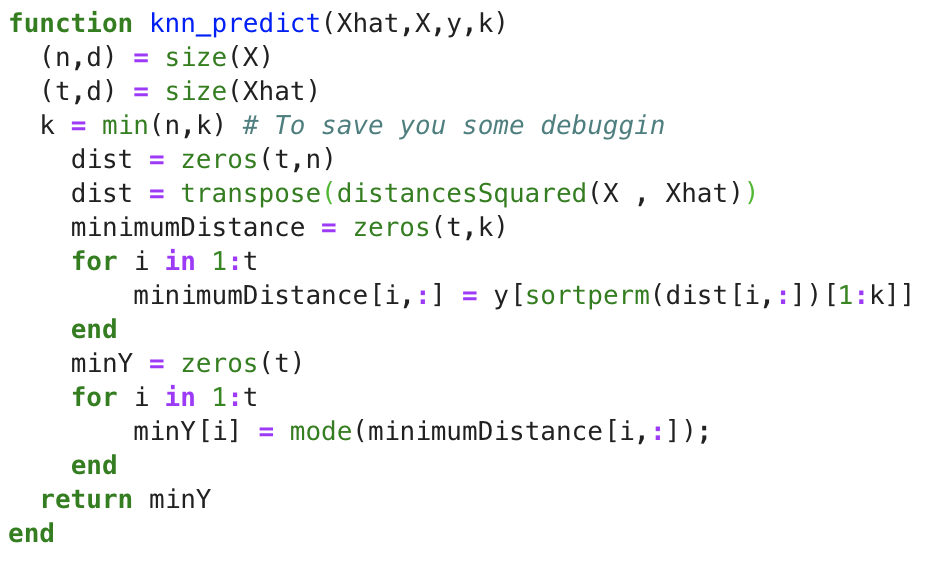
\includegraphics[width = 10cm]{Q3Predict.png}}
\item Report  the training and test error obtained on the \emph{citiesSmall.mat} dataset for $k=1$, $k=3$, and $k=10$. (You can use \emph{example\_knn.jl} to get started.) \ans{k = 1: Training Eror : 0, Test Error: 0.065 \\ k =3: Training Eror : 0.028, Test Error: 0.066 \\ k =10: Training Eror : 0.072, Test Error: 0.097  }
\item Hand in the plot generatied by {classifier2Dplot} on the \emph{citiesSmall.mat} dataset for $k=1$ on the training data. \item Why is the training error $0$ for $k=1$? \ans{\\ 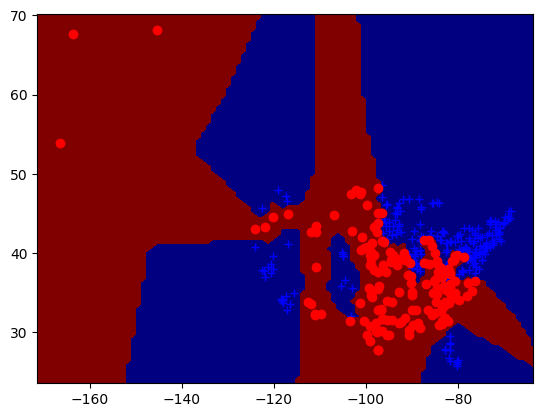
\includegraphics[width=10cm]{Q3KnnPredictionGraph.png}}
\item If you didn't have an explicit test set, how would you choose $k$? \ans{Use part of the training set as validation set.}
}
}

Hint: when writing a function, it is typically a good practice to write one step of the code at a time and check if the code matches the output you expect. You can then proceed to the next step and at each step test is if the function behaves as you expect. You can also use a set of inputs where you know what the output should be in order to help you find any bugs. These are standard programming practices: it is not the job of the TAs or the instructor to find the location of a bug in a long program you've written without verifying the individual parts on their own.

\subsection{Condensed Nearest Neighbours}

The file \emph{citiesBig1.mat} contains a version of this dataset with more than 30 times as many cities. KNN can obtain a lower test error if it's trained on this dataset, but the prediction time will be very slow. A common strategy for applying KNN to huge datasets is called \emph{condensed nearest neighbours}, and the main idea is to only store a \emph{subset} of the training examples (and to only compare to these examples when making predictions). A simple variation of this algorithm would be:

\begin{algorithm}[H]
 initialize subset with first training example\;
 \For{each  training example}{
  \eIf{the example is incorrectly classified by the KNN classifier using the current subset}{
   add the current example to the subset\;
   }{
   do \emph{not} add the current example to the subset (do nothing)\;
  }
 }
 \caption{Condensed Nearest Neighbours}
\end{algorithm}
You are provided with an implementation of this \emph{condensed nearest neighbours} algorithm in \emph{knn.jl}. 
\blu{
\enum{
\item The point of this algorithm is to be faster than KNN. Try running the condensed nearest neighbours (called ``cknn'' in the code) on the \emph{citiesBig1} dataset and report how long it takes to make a prediction. What about if you try to use KNN for this dataset? \ans{It will take about 16 seconds for KNN and about 0.62 seconds for CKNN}
\item Report the training and testing errors for condensed NN, as well as the number of training examples in the subset, on the \emph{citiesBig1} dataset with $k=1$. \ans{Training Error: 0.008, Test Error: 0.018 and the \# of the Training Example is 457}
\item Why is the training error with $k=1$ now greater than $0$? \ans{Because we are only checking once for each example in the dataset, if a new data point is added, it might also affect the previous point to be misclassified.}
\item If we entered the coordinates of Vancouver into the predict function, would it be predicted to be in a blue state or a red state? \ans{Blue}
\item If you have $s$ examples in the subset, what is the cost of running the predict function on $t$ test examples in terms of $n$, $d$, $t$, and $s$? \ans{O(sdt)}
\item Try out your function on the dataset \emph{citiesBig2}. Why are the  test error \emph{and} training error so high (even for $k=1$) for this method on this dataset? \ans{Because the more of the point is influenced by the points added later on, A possible solusion is to do the main loop more times, the training error decreased to 0.007 after 2 more iterations. }
}
}


\section{Random Forests}

 
 \subsection{Implementation}
 
The file \emph{vowels.jld} contains a supervised learning dataset where we are trying to predict which of the 11 ``steady-state'' English vowels that a speaker is trying to pronounce.

You are provided with a a \texttt{randomTree} function in \emph{randomTree.jl} (based on information gain). The random tree model differs from the decision tree model in two ways: 
it takes a bootstrap sample of the data before fitting and when fitting individual stumps it only considers $\lfloor \sqrt{d} \rfloor$ randomly-chosen features.\footnote{The notation $\lfloor x\rfloor$ means the ``floor'' of $x$, or ``$x$ rounded down''.}  
In other words, \texttt{randomTree} is the model we discussed in class that is combined to make up a random forest.

If you run \emph{example\_randomTree.jl}, it will fit both models to the dataset, and you will notice that it overfits badly.

\blu{
\enum{
\item If you set the \emph{depth} parameter to \emph{Inf}, why do the training functions terminate?
\item Why does the random tree model, using infoGain and a depth of \emph{Inf}, have a training error greater 0?
\item Create a function \texttt{randomForest} that takes in hyperparameters \texttt{depth} and \texttt{nTrees} (number of trees), and 
fits \texttt{nTrees} random trees each with maximum depth \texttt{depth}. For prediction, have all trees predict and then take the mode. Hand in your function. Hint: you can define an array for holding 10 \emph{GenericModel} types using:\\
\texttt{subModels = Array\{GenericModel\}(undef,10)}.
\item Using 50 trees, and a depth of $\infty$, report the training and testing error. Compare this to what we got with a single \texttt{DecisionTree} and with a single \texttt{RandomTree}. Are the results what you expected? Discuss. 
\item Why does a random forest typically have a training error of 0, even though random trees typically have a training error greater than 0?
}
}

\section{K-Means Clustering}

If you run the function \emph{example\_Kmeans}, it will load a dataset with two features and a very obvious clustering structure. It will then apply the $k$-means algorithm with a random initialization. The result of applying the algorithm will thus depend on the randomization, but a typical run might look like this:
(Note that the colours are arbitrary due to the label switching problem.)
But the `correct' clustering (that was used to make the data) is something more like this:

\subsection{Selecting among k-means Initializations}

If you run the demo several times, it will find different clusterings. To select among clusterings for a \emph{fixed} value of $k$, one strategy is to minimize the sum of squared distances between examples $x_i$ and their means $w_{y_i}$,
\[
f(w_1,w_2,\dots,w_k,y_1,y_2,\dots,y_n) = \sum_{i=1}^n \norm{x_i - w_{y_i}}_2^2 = \sum_{i=1}^n \sum_{j=1}^d (x_{ij} - w_{y_ij})^2.
\]
 where $y_i$ is the index of the closest mean to $x_i$. This is a natural criterion because the steps of k-means alternately optimize this objective function in terms of the $w_c$ and the $y_i$ values.
 
 \blu{\enum{
 \item Write a new function called \emph{kMeansError} that takes in a dataset $X$, a set of cluster assignments $y$, and a set of cluster means $W$, and computes this objective function. Hand in your code.
 \item Instead of printing the number of labels that change on each iteration, what trend do you observe if you print the value of \emph{kMeansError} after each iteration of the k-means algorithm?
 \item Using the \emph{clustering2Dplot} file, output the clustering obtained by running k-means 50 times (with $k=4$) and taking the one with the lowest error. Note that the k-means training function will run much faster if you set \texttt{doPlot = false} or just remove this argument.
 }}
 
 \subsection{Selecting $k$ in k-means}
 
 We now turn to the task of choosing the number of clusters $k$.
  
 \blu{\enum{
 \item Explain why the \emph{kMeansError} function should not be used to choose $k$.
 \item Explain why even evaluating the \emph{kMeansError} function on test data still wouldn't be a suitable approach to choosing $k$.
 \item Hand in a plot of the minimum error found across 50 random initializations, as you vary $k$ from $1$ to $10$.
 \item The \emph{elbow method} for choosing $k$ consists of looking at the above plot and visually trying to choose the $k$ that makes the sharpest ``elbow" (the biggest change in slope). What values of $k$ might be reasonable according to this method? Note: there is not a single correct answer here; it is somewhat open to interpretation and there is a range of reasonable answers.
 }}
 



\section{Very-Short Answer Questions}

\blu{Write a short one or two sentence answer to each of the questions below}. Make sure your answer is clear and concise.

\enum{
 \item What is a feature transformation that you might do to address a ``coupon collecting'' problem in your data? \ans{Discretization}
\item What is one reason we would want to look at scatterplots of the data before doing supervised learning? \ans{Because summary statistics may trick us.}
 \item When we fit decision stumps, why do we only consider $>$ (for example) and not consider $<$ or $\geq$? \ans{Because they will give the same result.}
\item What is a reason that the data may not be IID in the email spam filtering example from lecture? \ans{There might be the similar email from the same sender that will result in similarity and duplication which is not IID.}
\item What is the difference between a validation set and a test set? \ans{We will never look into the test set during our training. But we might use the validation set to determine our hyper-parameter. We are appropriate test error using validataion error and we are using test error to approximate the error in real life.}
\item Why can't we (typically) use the training error to select a hyper-parameter? \ans{Because this will interduce a bias that we are picking the best test error. Which means we might overfit the test data. }
\item What is an advantage and a disadvantage of using a large $k$ value in $k$-fold cross-validation. \ans{It will be more accurate with a higher k score. But it will also be more expensive}
\item Why is  naive Bayes called ``naive''? \ans{Because the naive bayes assumes each feature are independent, which means we are assuming $P(f_1,f_2,f_3 ... \cond y_i) = P(f_1\cond y_i)*P(f_2\cond y_i)*P(f_3\cond y_i)...$}
\item What is the effect of $k$ in KNN on the two parts (training error and approximation error) of the fundamental trade-off. Hint: think about the extreme values. \ans{If K is small, the training error will be samll, but the approximation error might be big. And with a higher K, the training error will be small but the approximation error will be big.} \ans{Add similar translations to the training data as additional training data.}
\item For any parametric model, how does increasing number of training examples $n$ affect the two parts of the fundamental trade-off. \ans{For paramatric model, increasing the training examples will decrease the training error and also the approximation error.}
\item Suppose we want to classify whether segments of raw audio represent words or not. What is an easy way to make our classifier invariant to small translations of the raw audio?
\item Both supervised learning and clustering models take in an input $x_i$ and produce a label $y_i$. What is the key difference?
\item In $k$-means clustering the clusters are guaranteed to be convex regions. Are the areas that are given the same label by KNN also convex?
}



\end{document}